%% Review of Scientific Instruments manuscript — custom induction furnace.
%% "Real person" restyled variant of paper.tex (R. Guymon, PR #3, 2026-07-14):
%% the whole manuscript rewritten in the style of the Extension-to-ceramics
%% section — no "~" (\sim) approximations (spelled out as "approximately" or
%% written as plain ranges) and no complicated run-on sentences (em-dash /
%% semicolon / colon splices split into short declarative sentences).
%% This is the live manuscript; paper.tex/paper.pdf are the frozen
%% pre-restyle record. Content differences from paper.tex: the
%% thermal-grooving panel is a main-text figure, the "Supplementary
%% Material" section follows the Conclusions, and four figures were
%% promoted from the SI to fill the 5-page limit (disassembled crucible,
%% vacuum/gas-handling photos, EBSD IPF maps, YSZ charge-stack schematic;
%% R. Guymon, PR #3, 2026-07-16). This file builds real_person_paper.pdf
%% (`make real`).
%% Editing pass (R. Guymon, PR #12, 2026-07-17): abbreviations and coined
%% terms (RF, YSZ, DAQ, EBSD, SEM, susceptor, charge stack, soak) are
%% defined only at first appearance, and figures use [tb] float placement
%% (not [ht]) so they sit at column tops/bottoms instead of interrupting
%% sentences or splitting paragraphs.
%% Correction (R. Guymon, PR #12, 2026-07-22): the KF40 flanges join the
%% quartz tube (the vacuum chamber) to the pyrometer housing and the vacuum
%% hardware; the charge stack is NOT flange-mounted -- it just sits inside
%% the chamber. The former "chamber stack" term was dropped accordingly.
%% Figure pass (S. Baird, PR #12, 2026-07-22): the system-overview schematic
%% and furnace photo are merged into one side-by-side figure (a)/(b) whose
%% caption states the key differentiators; the disassembled-crucible and
%% assembly-sequence figures are merged into fig_crucible_combined.png with
%% no caption text baked into the image (build_crucible_combined_figure.py);
%% the vacuum/gas-handling photos moved to the SI (Fig. S3); fig_ebsd.png is
%% rebuilt without in-image anneal titles (build_ebsd_figure.py) since panel
%% (b)'s run is unrecorded; the no-preparation EBSD observation is emphasized
%% in Sec. V; and "Ni4N5" is written "Ni (4N5)" with a 99.995 % gloss at
%% first use (text and figure caption).
%% Terminology pass (R. Guymon, PR #12, 2026-07-22): one name per stack.
%% "modernization stack" = the retrofit (control, vacuum, temperature
%% feedback); formerly drifted to "layer", "modernization layer", and bare
%% "stack". "sample stack" = specimen + susceptor + supports inside the
%% chamber; formerly "charge stack" and bare "stack". Every mention now uses
%% its concept's full name.
%%
%% Built on REVTeX 4.2 with the AIP substyles (`rsi` journal option) — the class
%% behind the official AIP Publishing template. Template files and the RSI/AIP
%% author guidelines are mirrored in paper/template/rsi/.
%%
\documentclass[%
 aip,
 rsi,%
 amsmath,amssymb,
 reprint,%
]{revtex4-2}

% REVTeX 4.2f (2022) patches LaTeX's tabular internals at \begin{document};
% those patches predate the 2023+ kernel/array rewrite (tagging-ready \@classz
% etc.) and fail with "Extra \or" errors. This manuscript uses standard
% booktabs/tabularx tables (not REVTeX's ruledtabular), so the patching is
% safely disabled.
\makeatletter
\def\switch@tabular{\class@info{REVTeX tabular patching disabled (post-2023 kernel)}}
\let\switch@array\switch@tabular
\makeatother

\usepackage{graphicx}
\usepackage{booktabs}
\usepackage{array}
\usepackage{tabularx}
\usepackage{xcolor}
\usepackage[colorlinks=true,allcolors=blue]{hyperref}
\usepackage{gensymb} % \degree, \celsius
\usepackage[htt]{hyphenat} % allow long \texttt{} paths to break across lines
\sloppy

% Draft notes: the status box and \todo markers are rendered only when the
% DRAFTNOTES macro is predefined. The default build is the clean PDF.
\newif\ifdraftnotes
\ifdefined\DRAFTNOTES\draftnotestrue\fi
\newcommand{\todo}[1]{\ifdraftnotes{\color{red}\textbf{[TODO: #1]}}\fi}

% Convenience column types for wide tables.
\newcolumntype{L}[1]{>{\raggedright\arraybackslash}p{#1}}
\newcolumntype{R}[1]{>{\raggedleft\arraybackslash}p{#1}}

% Validation figures generated by paper/build_validation_figures.py.
\graphicspath{{figures/}}

\begin{document}

\title{Retrofitting a commercial RF induction generator into a
computer-controlled, vacuum-integrated annealing system for reactive-metal
grain growth}

\author{Sterling G. Baird}
\affiliation{Department of Mechanical Engineering, Brigham Young University,
Provo, Utah 84602, USA}
\author{Ryan Weber}
\affiliation{Department of Mechanical Engineering, Brigham Young University,
Provo, Utah 84602, USA}
\author{Christopher Nyborg}
\affiliation{Department of Mechanical Engineering, Brigham Young University,
Provo, Utah 84602, USA}
\author{Ronnie Guymon}
\affiliation{Department of Mechanical Engineering, Brigham Young University,
Provo, Utah 84602, USA}
\author{Gage Erickson}
\affiliation{Department of Mechanical Engineering, Brigham Young University,
Provo, Utah 84602, USA}
\author{Oliver Johnson}% last author
\affiliation{Department of Mechanical Engineering, Brigham Young University,
Provo, Utah 84602, USA}
% K. Cole is acknowledged, not an author (S. Baird, PR #3, 2026-07-06/07-07).
% \todo{confirm author order (Weber vs. Nyborg) and middle initials}

\date{\today}

\begin{abstract}
High-temperature vacuum annealing near a metal's melting point drives
controlled grain growth, but it normally requires an expensive turn-key
vacuum induction furnace. We describe an open modernization stack (the
added control, vacuum, and temperature-feedback hardware and
software) that converts a bare commercial radio-frequency (RF) induction
generator into a computer-controlled,
vacuum-integrated annealing system with pyrometer feedback. The
modernization stack consists of analog power control through LabVIEW and a data-acquisition
(DAQ) device, dual-wavelength optical
temperature feedback, a high-vacuum quartz-tube chamber, and an in-house
machined graphite crucible that serves as a susceptor (an RF-absorbing
element that heats the charge it encloses) for metal specimens.
Because its only requirement is a monotonic analog power-control input,
the modernization stack transfers between generators; the reference build
uses a 6\,kW solid-state generator. The system produced a
fixed-geometry power--temperature calibration with $R^2 = 0.991$ over
1200--1400\,\celsius. Eight nickel anneals at 1200\,\celsius{} for 12\,h
reproduced their soak temperature (the constant-temperature hold) to
$1201.2 \pm 1.3$\,\celsius, and soaks up to
40\,h at 1325\,\celsius{} remained stable. In the annealed nickel, optical
metallography and scanning electron microscopy (SEM) resolve equiaxed
grains and deep thermal grooves, several spanning the full sheet
thickness; electron backscatter diffraction (EBSD) maps index hundreds of
grains, quantifying grain size and texture.
A modified sample stack (the stacked specimen, susceptor, and supports
inside the chamber) extends the furnace to non-coupling
ceramics, demonstrated by coarsening yttria-stabilized zirconia (YSZ)
grains in 45\,min at 2500\,\celsius.
Complete design
files, bill of materials, control software, and data are openly
available.
\end{abstract}

\keywords{induction furnace; grain growth; vacuum annealing; LabVIEW;
pyrometer; open-source hardware}

\maketitle

\ifdraftnotes
\noindent\fbox{\parbox{\linewidth}{\small\textbf{Status:} restyled
("real person") variant of paper.tex; content is identical, prose is
rewritten in the Extension-to-ceramics style. \todo{}-marked items flag
values that still need to be confirmed before submission.}}
\fi

%==============================================================
\section{Introduction}
%==============================================================

High-temperature annealing near a metal's melting point drives controlled
grain growth. This is central to studying microstructure--property
relationships in metals such as nickel and
iron~\cite{liu2021studyofgrain,mohrbacher2026applicationofmicroalloying,alogab2007theinfluenceof,tian2009experimentalandsimulation,moore2017graincoarseningbehaviour}.
Growing grains without oxidizing the sample requires temperatures of 1400 to
1500\,\celsius{} along with high vacuum or an inert
atmosphere~\cite{zhornyak1982reductionanddecarburization,muramatsu2005gascontaminationdue}.
Commercial vacuum induction furnaces that meet these requirements are
closed, turn-key systems costing \$50k to \$200k or more. Resistive tube and
box furnaces reach lower temperatures with slower ramps, and they offer no
susceptor route to charges that do not couple to the RF field. Bare
industrial induction generators are widely available, but they ship without
vacuum, optical temperature feedback, or computer setpoint control.

This work adds that missing modernization stack. A bare RF induction
generator~\cite{rudnev2017handbookofinduction,lucia2014inductionheatingtechnology}
is retrofitted into a full annealing system with computer power control,
closed-loop optical temperature feedback, a high-vacuum quartz-tube chamber,
and a machined graphite crucible that doubles as a susceptor. The
modernization stack is deliberately generator-agnostic. Its only requirement is an analog
power-control input, such as 4--20\,mA or 0--5\,V, with a monotonic
command-to-power response. The pyrometer feedback and
proportional--integral--derivative (PID) calibration absorb
any nonlinearity in that response. The generator internals are not
reproduced, so a compatible generator needs to be supplied. The graphite
crucible couples strongly to the RF field and serves the metal grain-growth
charges. Non-coupling ceramics such as YSZ
use a modified sample stack in
which graphite or tantalum serves as the susceptor, chosen for chemical
compatibility with the specimen (Sec.~\ref{sec:ysz}).

The reproducible build documented here is anchored on a current, USA-sourced
6\,kW solid-state generator whose controller accepts a standard 4--20\,mA
power setpoint. The package of generator, heating head, controller, and
chiller was quoted at approximately \$16.5k. The retrofit components are
itemized in the bill of materials in the supplementary material. This is a
small fraction of turn-key cost, in a form the user can repair and modify.

%==============================================================
\section{System design and description}
%==============================================================

The system comprises five subsystems (Fig.~\ref{fig:overview}(a)).
Figure~\ref{fig:overview}(b) shows the assembled system at operating power.

% TODO (R. Guymon): make the label text in the schematic (a) and the photo
% call-outs (b) the same font and font size (S. Baird, PR #12, 2026-07-22).
\begin{figure*}[tb]
\centering
\begin{minipage}[b]{0.60\textwidth}
\raggedright{\textbf{(a)}}\\[1pt]
\centering
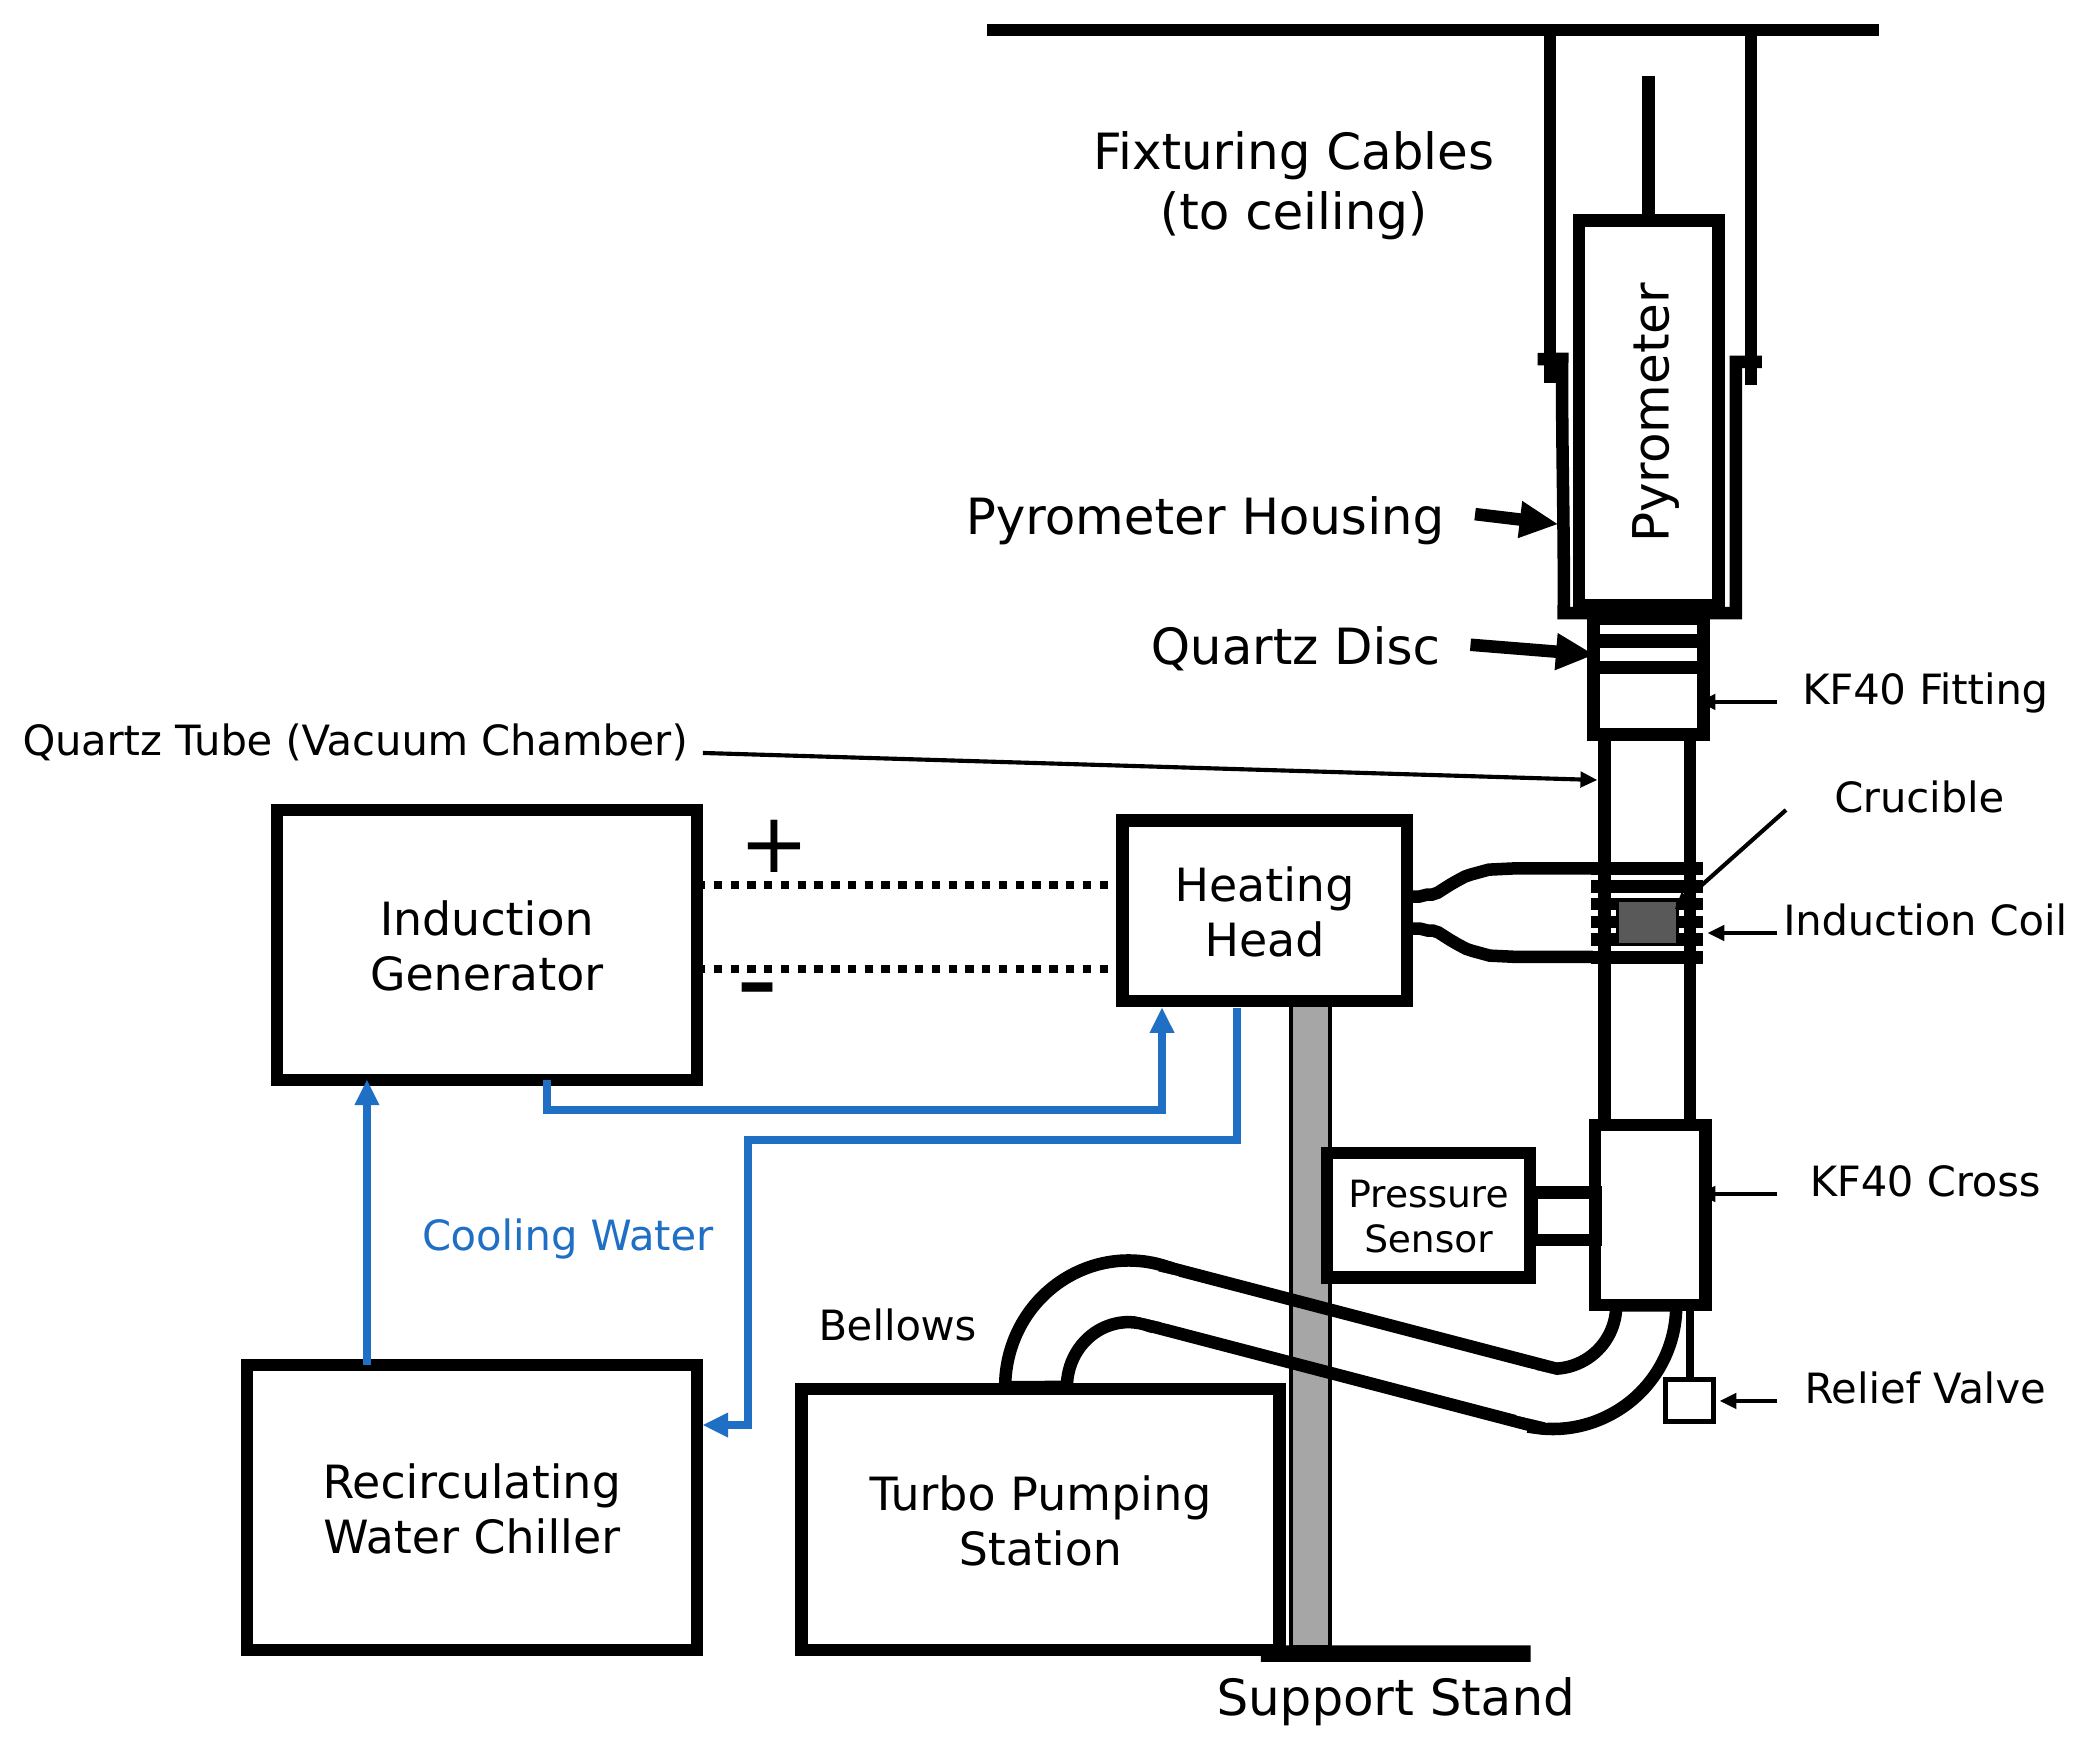
\includegraphics[width=\linewidth]{fig_system_overview_v2.png}
\end{minipage}\hfill
\begin{minipage}[b]{0.365\textwidth}
\raggedright{\textbf{(b)}}\\[1pt]
\centering
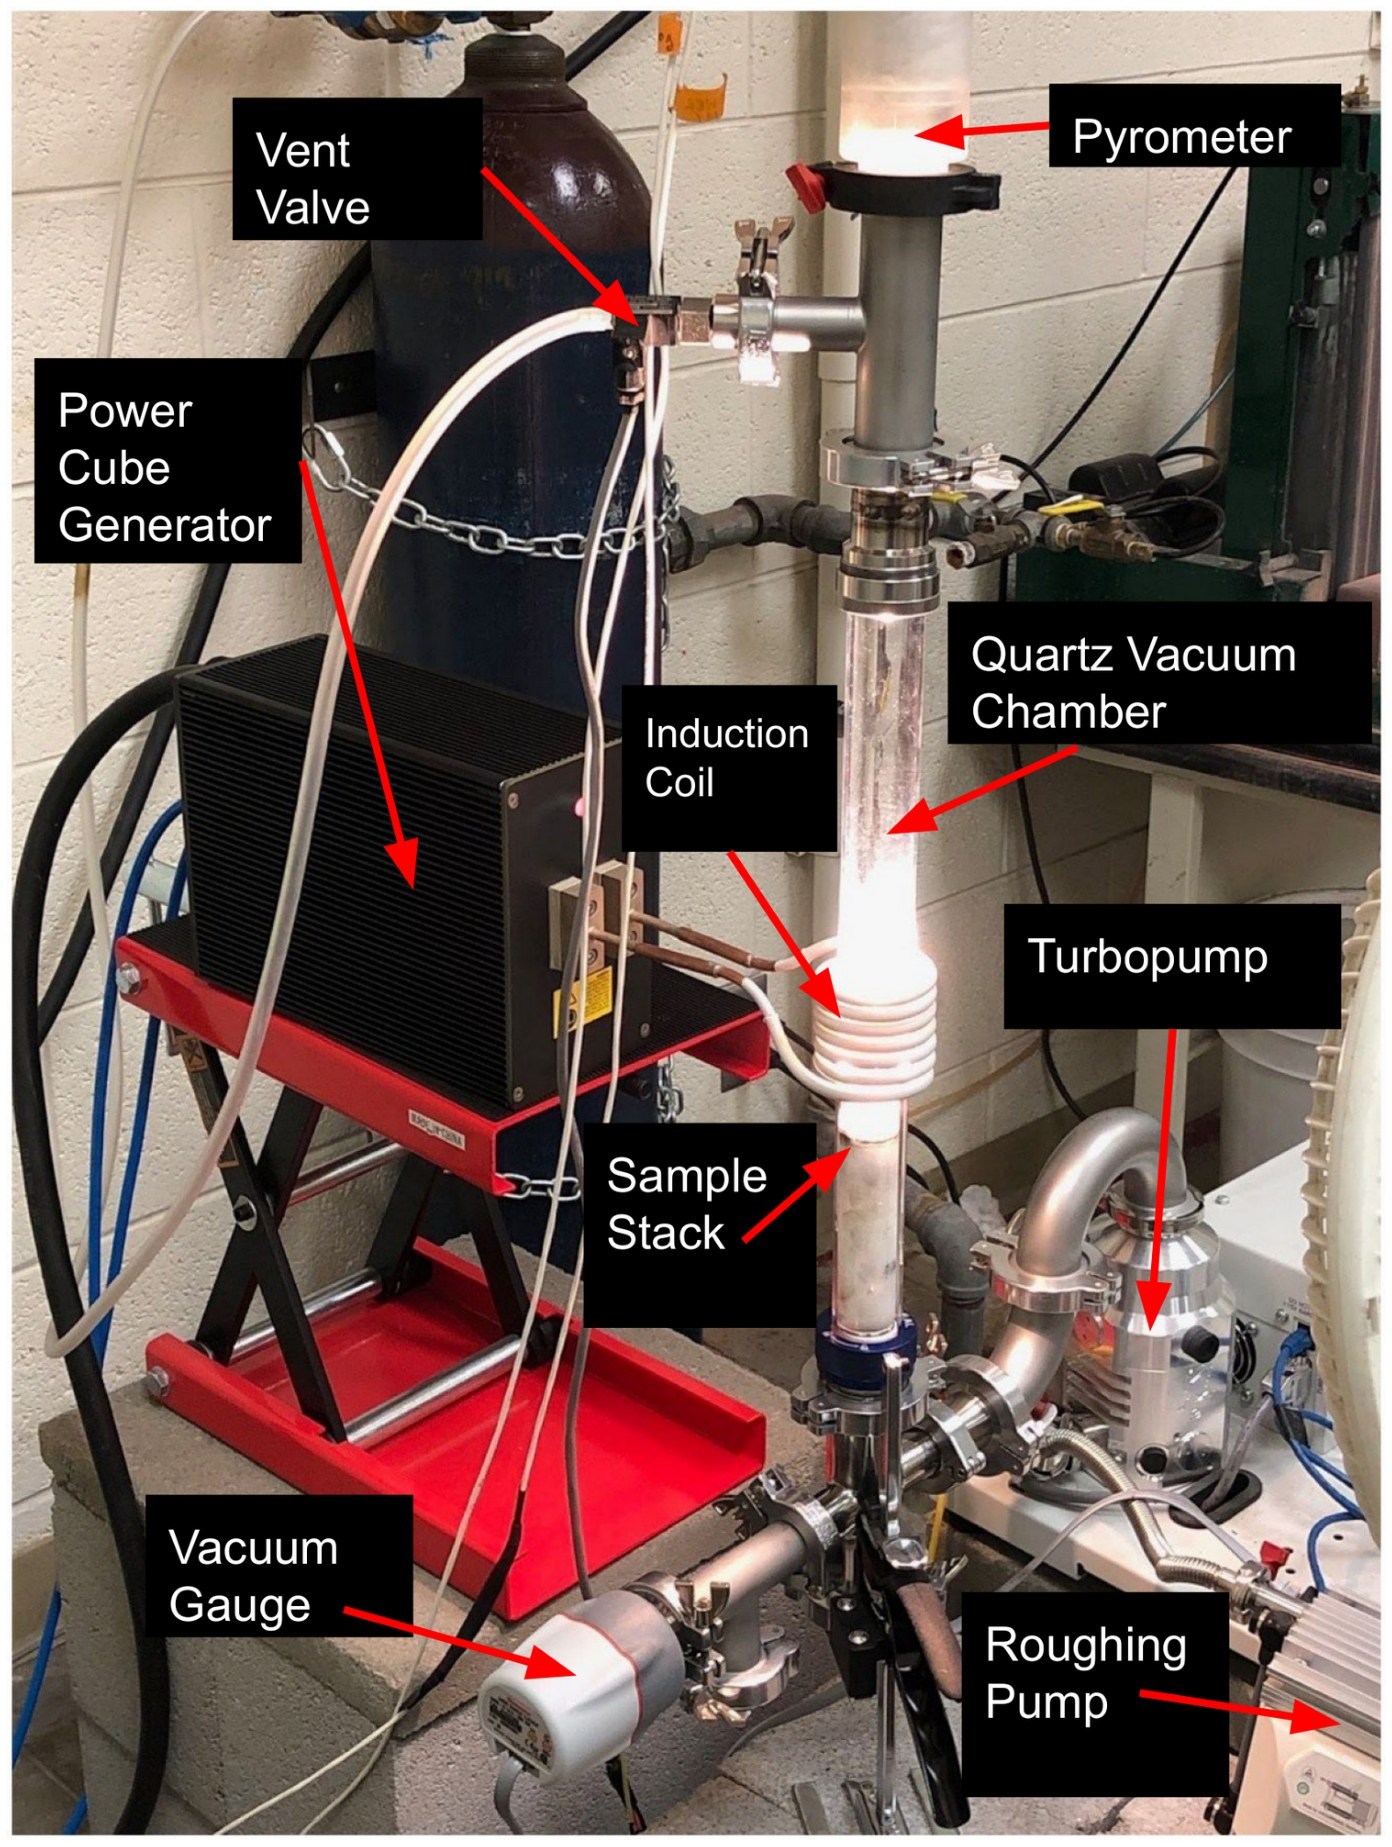
\includegraphics[width=\linewidth]{fig_furnace_photo.jpg}
\end{minipage}
\caption{The annealing system. (a)~System overview. The generator drives the
liquid-cooled heating head and work coil around the vertically suspended
quartz-tube chamber. The quartz tube is joined by KF40 flanges to the
ceiling-suspended pyrometer housing above and to the vacuum hardware below.
An overpressure relief valve and a flexible bellows lead past the pressure
sensor to the turbo pumping station. (b)~The assembled, functioning furnace
with the main components labeled. This shows the quartz chamber glowing at
the sample-stack position. The pyrometer sights down the chamber axis, and
the vent valve admits the argon backfill. The gauge, turbopump, and
separately supported roughing pump complete the vacuum path. Relative to
closed turn-key vacuum induction furnaces, this design costs far less, is
modular (hand-clamped KF-flanged vacuum hardware and an interchangeable
sample stack), and is transparent (open LabVIEW control software and design
files), and it reaches a high-purity annealing environment by pumping the
chamber to high vacuum and then backfilling with flowing argon.}
\label{fig:overview}
\end{figure*}

The heating subsystem is a 6\,kW solid-state induction generator driving a
liquid-cooled copper work coil. The coil is approximately 3\,in tall and
2.5\,in in inner diameter, with 6.5 turns tuned to the sample
stack~\cite{vankan2024electromagneticinductionheating,xu2026designandoptimization}.
The coil conductors carry both the RF current and the coolant. Ethylene
glycol coolant flows in series from the chiller through the generator and
then through the heating head and work coil before returning to the chiller.
The vacuum and gas subsystem starts from the 35\,mm inner-diameter
fused-quartz tube that forms the chamber. The tube connects through a KF40
flange (a standard clamp-sealed vacuum flange) and a flexible bellows to a
compact turbo pumping station that
reaches 10$^{-6}$ to 10$^{-8}$\,Torr. A manual vent valve fed from an
inert-gas regulator allows controlled venting and
backfilling~\cite{kanda2007developmentofhightemperature,inaba1986effectsofthe}.
The atmosphere matters for graphite-crucible anneals. The best results were
achieved by pumping to high vacuum and then backfilling with argon through
the vent valve. The chamber was purged first, and a constant argon flow of
20 standard cubic centimeters per minute (SCCM) was then maintained for the
duration of the anneal. The nickel
grain-growth anneals reported below all ran under this continuous flow.
Heating under vacuum alone tended to sublime graphite onto the chamber
walls. The highest-temperature ceramic work (Sec.~\ref{sec:ysz}) used the
same continuous argon supply, with the chamber evacuated and then filled
with argon while the turbopump was running. This helped avoid oxidation
during heating.

Temperature is sensed optically. A dual-wavelength ratio
pyrometer~\cite{tapetado2016twocolorpyrometerfor,belikov2024fastmultiwavelengthpyrometer}
with an 800 to 2500\,\celsius{} sensing range views the sample through a
KF40 optical window. This provides a non-contact signal that is robust to
emissivity changes and to the RF field that would corrupt
thermocouples~\cite{ham2016insituspectralemissivity,suleiman2025improvingpyrometryof,usamentiaga2014infraredthermographyfor}.
Control is implemented in LabVIEW, with virtual instruments (VIs) for
manual control, automated
ramping, PID tuning, and email alerts. The DAQ device's
0--5\,V analog output
drives a voltage-to-current loop conditioner, and the conditioner's
4--20\,mA output lands on the generator's power-setpoint input. The
pyrometer's analog output returns to a DAQ input, which closes the PID loop.
Below the pyrometer's detection floor of approximately 700\,\celsius, the VI
ramps open-loop. Once the pyrometer returns a sustained valid reading,
control hands over to closed-loop PID on the optical
temperature~\cite{meng2023designofvacuum,rapoport2006optimalcontrolof}.
Mechanically, a bolted support stand carries the generator's heating head
and centers the work coil on the crucible position. The vacuum chamber
itself has no support stand. The quartz tube and the vacuum hardware below
it are joined by KF40 flanges to the pyrometer housing, which is suspended
from the ceiling by cables, so the vertical column of vacuum hardware hangs
from above. The sample stack is not attached to any of these flanges. It
simply sits inside the quartz tube.

Metal charges in the graphite crucible reach the nickel and iron
grain-growth range of 1400 to 1500\,\celsius, with demonstrated soaks
from minutes to 40\,h. The modified ceramic sample stack extends the working
range to 2500\,\celsius. The modernization stack transfers to
any generator that exposes a monotonic analog power input, supports a
liquid-cooled head and coil of the documented geometry, delivers enough RF
power for the target charge, and allows electrical isolation of the DAQ and
control path. When porting, the command scaling, calibration, PID gains,
alignment, and interlock behavior are re-established.

\subsection{Graphite crucible / susceptor}

Metal specimens are held in a two-piece graphite crucible machined in-house
from 3000\,\celsius-grade graphite stock. It consists of a cup body and a
lidded cap with a central bore, which contains the charge while leaving an
optical path for the pyrometer. Figure~\ref{fig:crucible}(a) shows the
disassembled parts. The graphite couples strongly to the
induction field and acts as a susceptor, heating the contained metal
specimen by conduction and radiation. The specimen is sandwiched between two
alumina discs in the cup, the lid seats on top, and a sapphire window closes
the lid bore (Fig.~\ref{fig:crucible}(b--d)). Sapphire is used for the
window to increase transmittance in the wavelength ranges emitted from the
sample relative to the pyrometry. When fully assembled the crucible stands
13\,mm tall, and the measured dimensions of every piece are given in the
supplementary material. Inside the vacuum chamber the crucible rests on an
alumina support rod that positions it at coil height.
% TODO (ask Chris): what does the alumina support rod itself rest on at its
% lower end -- just the metal vacuum tubes/fittings below the quartz tube? Crucibles are repaired
with graphite cement rather than discarded. The crucible primarily serves
the metal grain-growth charges. Graphite also works as a susceptor for some
ceramic charges when the contact chemistry permits.
Sec.~\ref{sec:ysz} describes how a compatible susceptor is selected for
refractory ceramics.

\begin{figure}[tb]
\centering
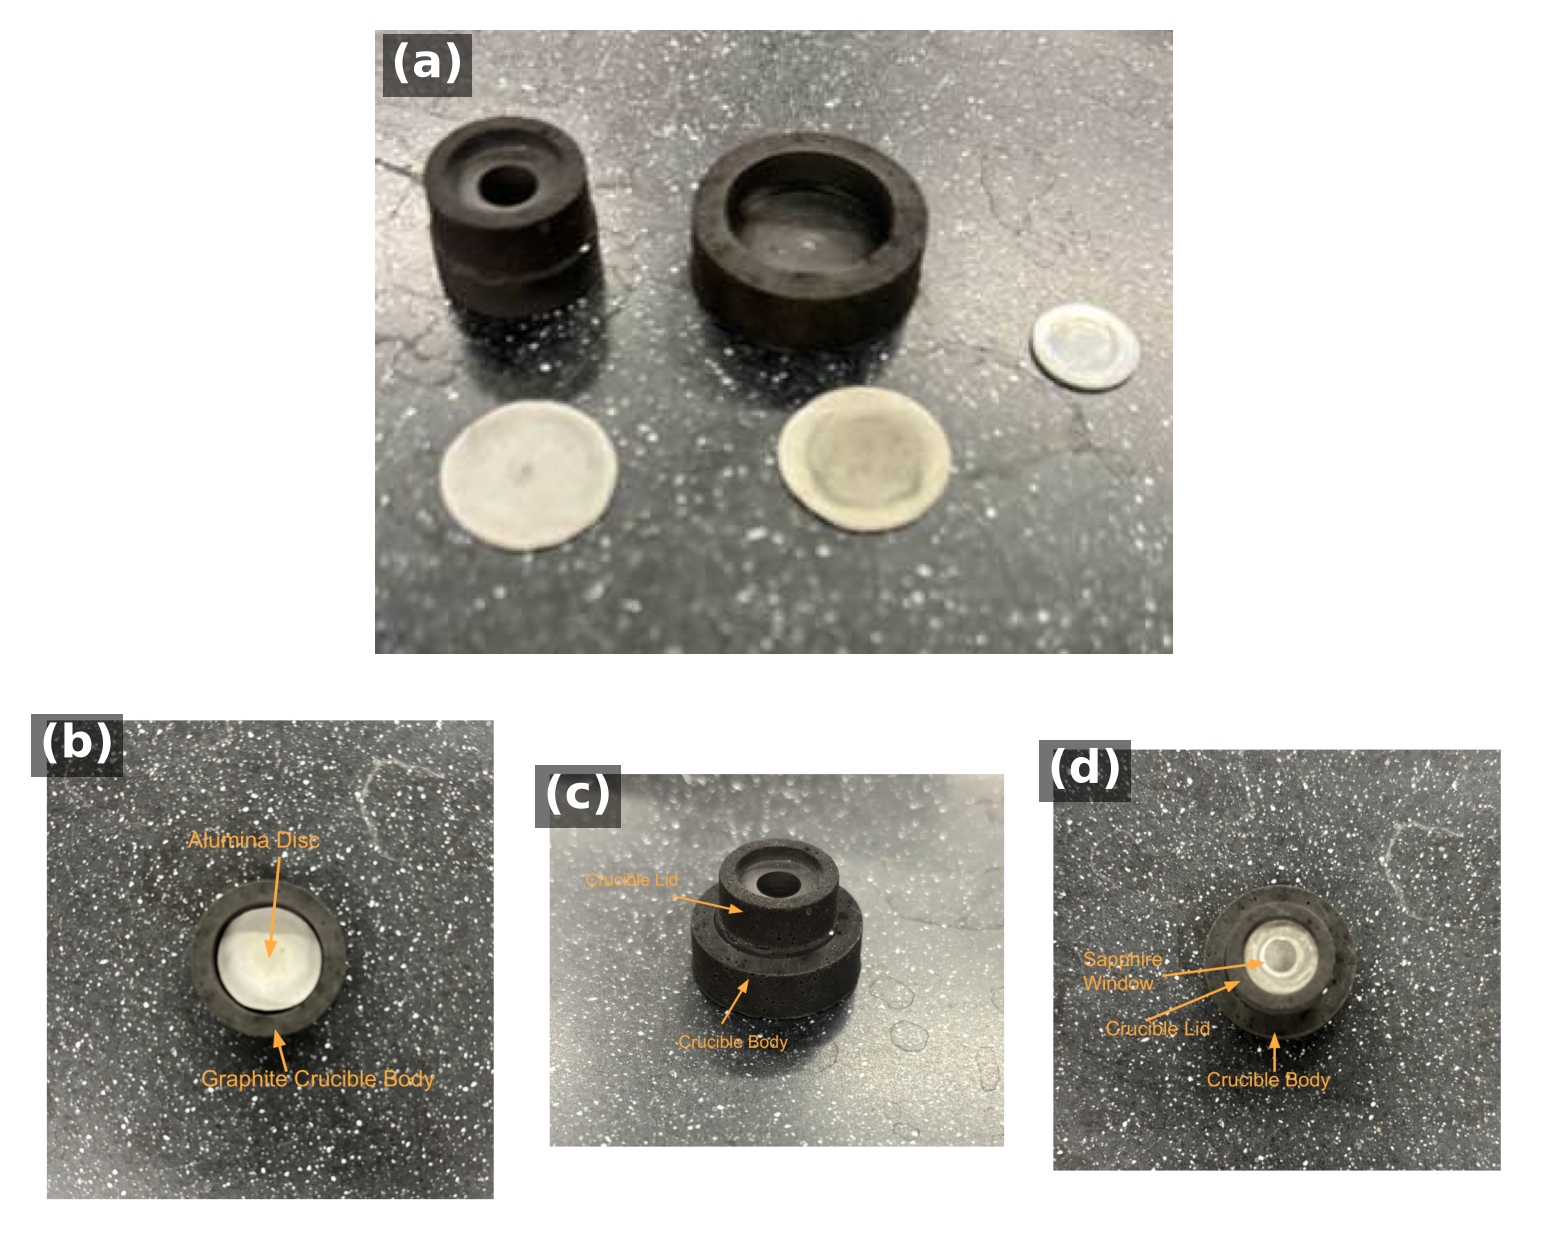
\includegraphics[width=0.92\linewidth]{fig_crucible_combined.png}
\caption{The two-piece graphite crucible/susceptor used for the nickel
anneals reported in this work. (a)~Fully disassembled. Top left is the
crucible lid, top middle is the bottom of the crucible that acts as the
specimen carrier, far right is the sapphire window, bottom left and middle
are the alumina sample-surrounding sheets. (b--d)~Specimen-loading sequence.
(b)~The specimen is placed between two alumina sheets in the crucible body.
(c)~The graphite lid is seated on top. (d)~The sapphire window closes the lid
bore, leaving an optical path for the pyrometer.}
\label{fig:crucible}
\end{figure}

%==============================================================
\section{Construction and operation}
%==============================================================

Following the heating path, the generator's heating head mounts on an
adjustable platform on the bolted support stand so the coil centers on the
crucible position of the vertically suspended quartz tube. The vacuum path
begins at the quartz tube, whose open end terminates in a KF40 flange closed
by a 55\,mm quartz optical disc. Every flanged joint compresses an elastomer
O-ring carried on a centering ring, so the vacuum hardware assembles with
hand-tightened clamps and no tools. These seals support the 10$^{-6}$ to
10$^{-8}$\,Torr operating vacuum. From the bottom of the vacuum column, a tee
carries a 0.5\,psi overpressure relief valve that protects the quartz tube
during backfilling. A flexible bellows continues through the wide-range
vacuum gauge to the turbo pumping station. The roughing pump sits on a
separate support, mechanically decoupled so its vibration does not reach the
chamber or the pyrometer sight line. Photographs of the pumping station as
installed, together with the relief valve at the base of the vacuum column,
are given in the supplementary material. On the gas path, the argon regulator
feeds the manual vent valve. A mass flow controller between them is helpful
when continuous inert gas flow is required. On the control path, electrical
isolation is maintained between the DAQ wiring and the generator interface.
Manual control is verified before automated ramping and soaking are enabled.

A run begins with the chamber vented, which is done only after the turbo
pump has stopped spinning. The specimen is loaded into the crucible
(Fig.~\ref{fig:crucible}(b--d)), the sample stack is lowered into the
quartz tube, and the chamber is pumped down. The LabVIEW profile ramps open-loop below the pyrometer
floor, hands over to closed-loop PID, and runs the programmed soak.
Afterwards the sample cools under vacuum, and the chamber is vented only
once the turbo pump has stopped.

%==============================================================
\section{Performance validation}
%==============================================================

The furnace has completed more than one hundred logged anneals of Ni200 and
Ni (4N5, i.e., 99.995\,\% purity) nickel charges, and of palladium
thermal-evaporation charges, at 900 to
1400\,\celsius, with soaks from minutes to 40\,h. The supplementary material
links each result below to its underlying run log.

For one fixed configuration of Ni (4N5) specimen, quartz tube, graphite
crucible, and optics, four steady-state anneals spanning 1200 to
1400\,\celsius{} give a monotonic relation between the soak-mean analog
power command and the soak-mean pyrometer temperature. The relation is well
described by $T = 931 + 632\,I$, with $T$ in \celsius{} and $I$ in mA, and
$R^2 = 0.991$. The offset shifts with charge and optical configuration, so
this is an operational calibration for a given setup, not a universal
command--temperature law. A Ni (4N5) anneal at a nominal 1300\,\celsius{} and
12\,h condition serves as the representative closed-loop run, and its trace
is given in the supplementary material. The soak held
$1302.1 \pm 3.0$\,\celsius{} over the 12\,h plateau. The 10--90\,\% rise
time was approximately 1135\,s, the overshoot was approximately
12\,\celsius, and the drift was a negligible $-0.02$\,\celsius{} per hour.

Eight Ni (4N5) anneals at a nominal 1200\,\celsius{} and 12\,h condition were
run under the same gas-flow configuration. They reproduced their soak
temperature to $1201.2 \pm 1.3$\,\celsius, a coefficient of variation of
0.11\,\%. Long-duration stability was demonstrated with two Ni200 anneals at
1325\,\celsius. The first held for 20\,h at $1326.5 \pm 1.5$\,\celsius{}
with a drift of $-0.004$\,\celsius{} per hour, and the second held for
40\,h. Figures for both are in the supplementary material. Reported
temperatures are closed-loop ratio-pyrometer readings in a fixed optical
geometry. Absolute specimen temperature still depends on emissivity and
surface
condition~\cite{ham2016insituspectralemissivity,giulietti2025spectralemissivitymeasurement,kieruj2016determinationofemissivity}.

%==============================================================
\section{Microstructural validation}
%==============================================================

The furnace exists to change microstructure, so the decisive test is what
the anneals do to real specimens. A striking feature of that test is that it
required no metallographic sample preparation at all. The EBSD specimens
shown here were never ground, polished, or etched. Each was pulled directly
from the furnace chamber and placed directly into the EBSD chamber.
Figure~\ref{fig:kikuchi} shows a raw EBSD pattern, also called a Kikuchi
pattern, from such an unprepared furnace-annealed nickel specimen,
reproduced exactly as the EBSD detector saved it during orientation mapping.
Even at the coarse $8\times8$ binning used for mapping, the bands and zone
axes are crisply resolved. EBSD diffracts from only the top few tens of
nanometers of the surface, so patterns of this quality from an as-annealed
surface indicate that the high-vacuum and flowing-argon environment left the
surface essentially free of the oxide film and near-surface deformation that
metallographic preparation normally exists to remove.
% Mechanism/precedent literature for the no-preparation EBSD observation is
% being gathered via an Edison Scientific literature task (PR #12,
% 2026-07-22, task e646f435-cd6f-4489-b67d-5ca6b5a0c19b; see
% paper/ebsd_noprep_query/).
Inverse-pole-figure maps built
from such patterns resolve hundreds of indexed grains per specimen
(Fig.~\ref{fig:ebsd}). Each indexed color in the map is a crystallographic
orientation, so a single map records both the grain sizes and the texture of
the annealed specimen. Thermal
grooving is itself a record of the anneal. Figure~\ref{fig:grooving} shows
edge-on views of a Ni (4N5) specimen annealed at 1200\,\celsius{} for 12\,h and
cleaned only ultrasonically. The grooves are deep, and several boundaries
traverse the full sheet thickness. This is a step toward columnar grain
structures~\cite{zhang2007dynamicsandmechanism}.

\begin{figure}[tb]
\centering
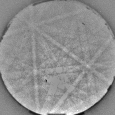
\includegraphics[width=0.36\linewidth]{fig_kikuchi_raw.jpg}
\caption{Raw EBSD Kikuchi pattern from a furnace-annealed nickel specimen
that received no sample preparation whatsoever --- no grinding, polishing,
or etching. The specimen was pulled directly from the furnace chamber and
placed directly into the EBSD chamber. The pattern is reproduced exactly as
saved by the EBSD detector during orientation mapping (the detector's
$8\times8$-binned output). Even so, the crisply resolved bands and zone axes
index directly to the nickel lattice.}
\label{fig:kikuchi}
\end{figure}

\begin{figure}[tb]
\centering
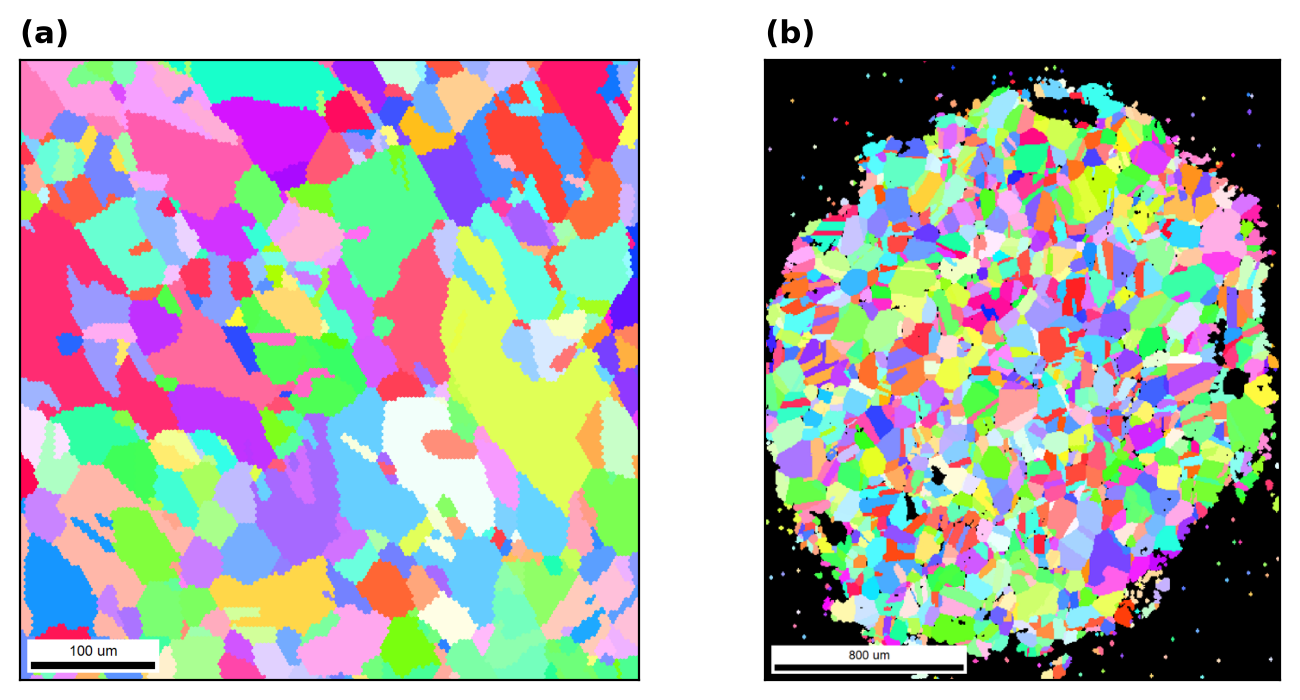
\includegraphics[width=0.94\linewidth]{fig_ebsd.png}
% Panel anneal conditions are deliberately omitted here: the (a) specimen's
% run is linked in SI Table S1, but the (b) specimen (Ni4N5_069) has no
% run-log linkage in the parsed set, and the recipe should appear for both
% panels or neither (S. Baird, PR #12, 2026-07-22).
% TODO (confirm with S. Baird): at which step the (b) specimen was masked,
% so the caption's masking wording can be made more specific.
\caption{EBSD inverse-pole-figure (IPF) orientation maps of two
furnace-annealed Ni (4N5, 99.995\,\% purity) specimens, rendered from the
recorded EBSD scans. Neither specimen received any sample preparation.
(a)~A furnace-annealed specimen (100\,\textmu m scale bar). (b)~A second
furnace-annealed specimen (800\,\textmu m scale bar). This specimen was
masked, which is why indexed points fill only the circular unmasked region
against the black surround. The maps resolve hundreds of grains for
grain-size and texture analysis. The supplementary material links each
specimen to its furnace run.}
\label{fig:ebsd}
\end{figure}

\begin{figure}[tb]
\centering
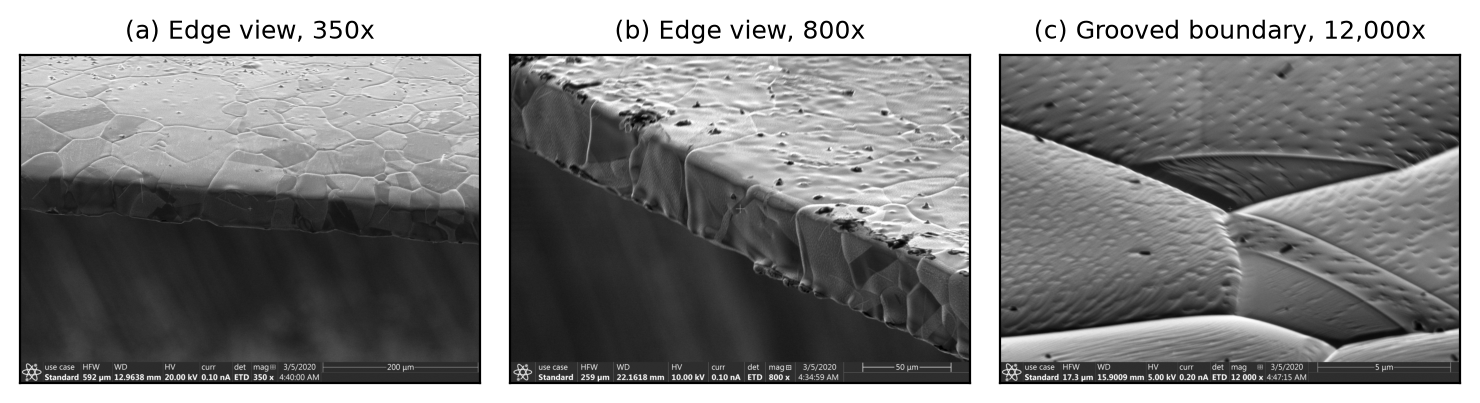
\includegraphics[width=0.92\linewidth]{fig_grooving.png}
\caption{Grain-boundary thermal grooving on a Ni (4N5) specimen after a
1200\,\celsius{} / 12\,h anneal, imaged edge-on in the as-annealed condition
after only an ultrasonic ethanol clean. (a)~Edge view at 350$\times$
(200\,\textmu m scale bar). Several grain boundaries traverse the full sheet
thickness. (b)~Edge and top surface at 800$\times$ (50\,\textmu m scale
bar). The grooves outline the surface grain structure. (c)~A single grooved
boundary at 12{,}000$\times$ (5\,\textmu m scale bar). The deep trench
develops as grain-boundary energy equilibrates against surface energy at the
soak temperature.}
\label{fig:grooving}
\end{figure}

Figure~\ref{fig:microstructure} shows the microstructure such an anneal
produces for a Ni (4N5) specimen soaked 20\,h at 1300\,\celsius{} under the
constant 20\,SCCM argon flow, with a measured soak of approximately
1301\,\celsius.
The optical grain map resolves an equiaxed grain network delineated by
thermal grooving alone. Grain-size measurements were made directly in the
image against its 200\,\textmu m scale bar. The SEM
detail resolves an
individual boundary groove at the micrometer
scale~\cite{bramfitt2001metallographersguidepractice}.

\begin{figure}[tb]
\centering
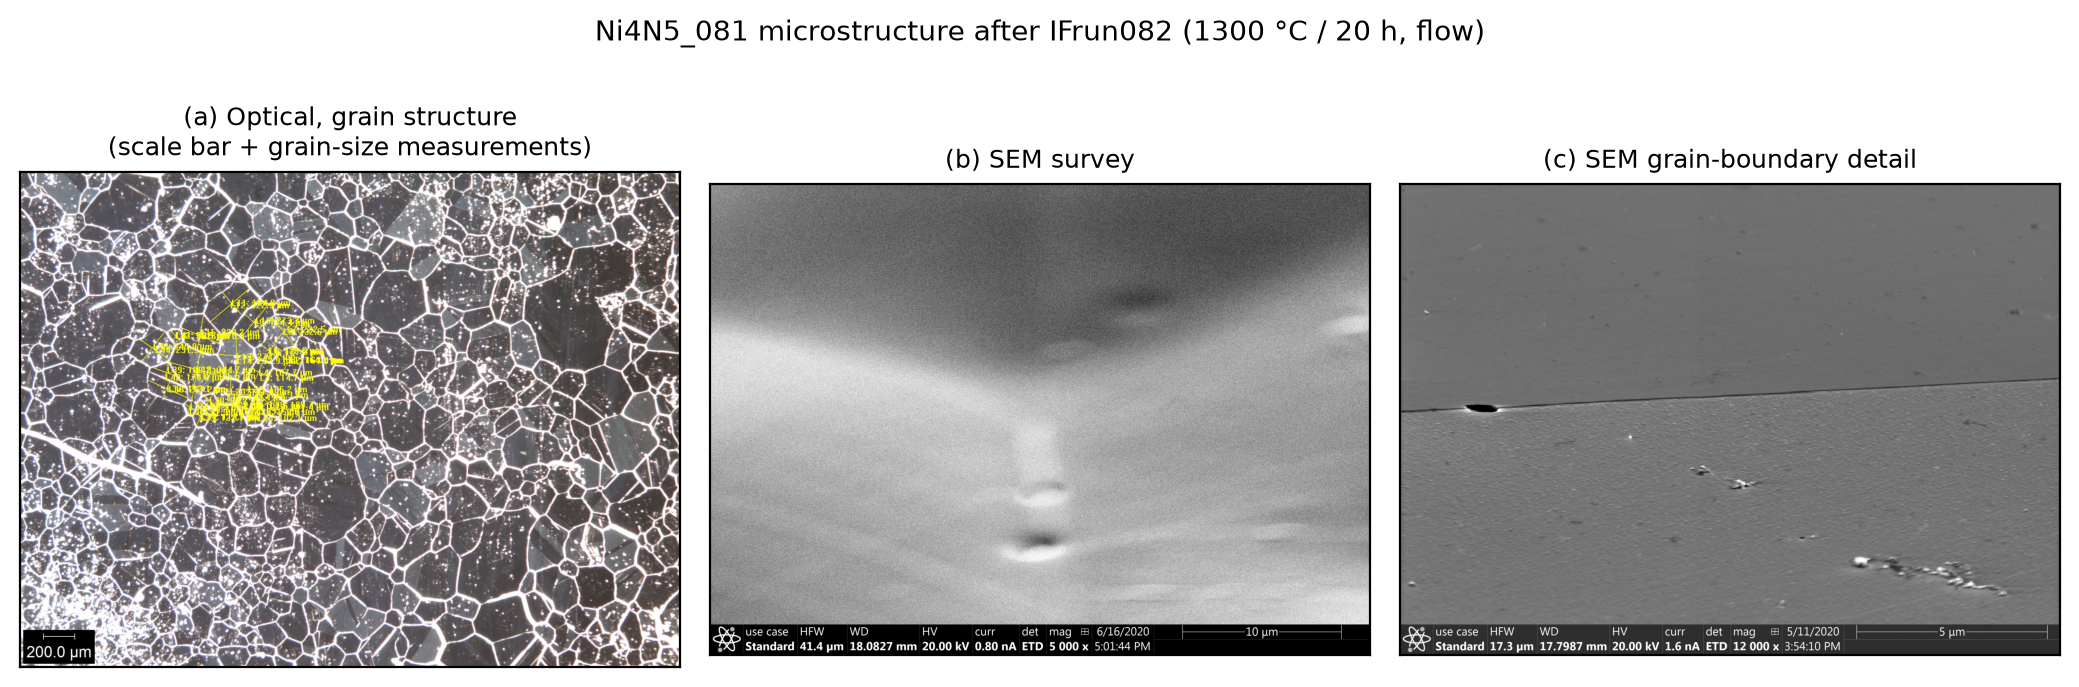
\includegraphics[width=0.68\linewidth]{fig_microstructure.png}
\caption{Microstructure of a Ni (4N5) specimen after a
1300\,\celsius{} / 20\,h anneal under a constant 20\,SCCM argon flow.
(a)~Optical grain
map with in-image grain-size measurements (200\,\textmu m scale bar);
(b)~high-magnification SEM grain-boundary detail.}
\label{fig:microstructure}
\end{figure}

\subsection{Extension to ceramic charges: YSZ}
\label{sec:ysz}

The same induction furnace can also be used to process refractory ceramics
by modifying only the materials directly in contact with the specimen while
leaving the generator, vacuum system, pyrometer, cooling system, and control
software unchanged. Materials that do not couple directly to the RF field
require a susceptor.
At the temperatures required for grains to coarsen on refractory ceramics,
the primary consideration in selecting a susceptor is its chemical
compatibility with the specimen and surrounding support materials rather
than its RF heating performance. Graphite and tantalum both serve
effectively as susceptors, with the preferred choice depending on the
operating temperature and the materials in contact with the susceptor.

Grain growth in refractory ceramics follows Arrhenius kinetics and is
therefore highly sensitive to annealing temperature. For the 8\,mol\% YSZ
specimens investigated here, grain growth from approximately 10\,\textmu m
to 90\,\textmu m required 228\,h at 1600\,\celsius{} in a conventional box
furnace, whereas comparable grain growth was achieved in only 45\,min at
2500\,\celsius{} using the induction furnace
(Fig.~\ref{fig:graingrowth}). Achieving these temperatures required only
minor modifications to the sample stack
(Fig.~\ref{fig:ysz-stack}). For example, direct contact
between graphite and alumina was eliminated because they undergo a eutectic
reaction that lowers the interface melting temperature to approximately
1800\,\celsius. This was accomplished by introducing a boron nitride
diffusion barrier between the two materials. Alternatively, replacing the
graphite with tantalum avoids this compatibility issue while still
providing efficient RF coupling.

\begin{figure}[tb]
\centering
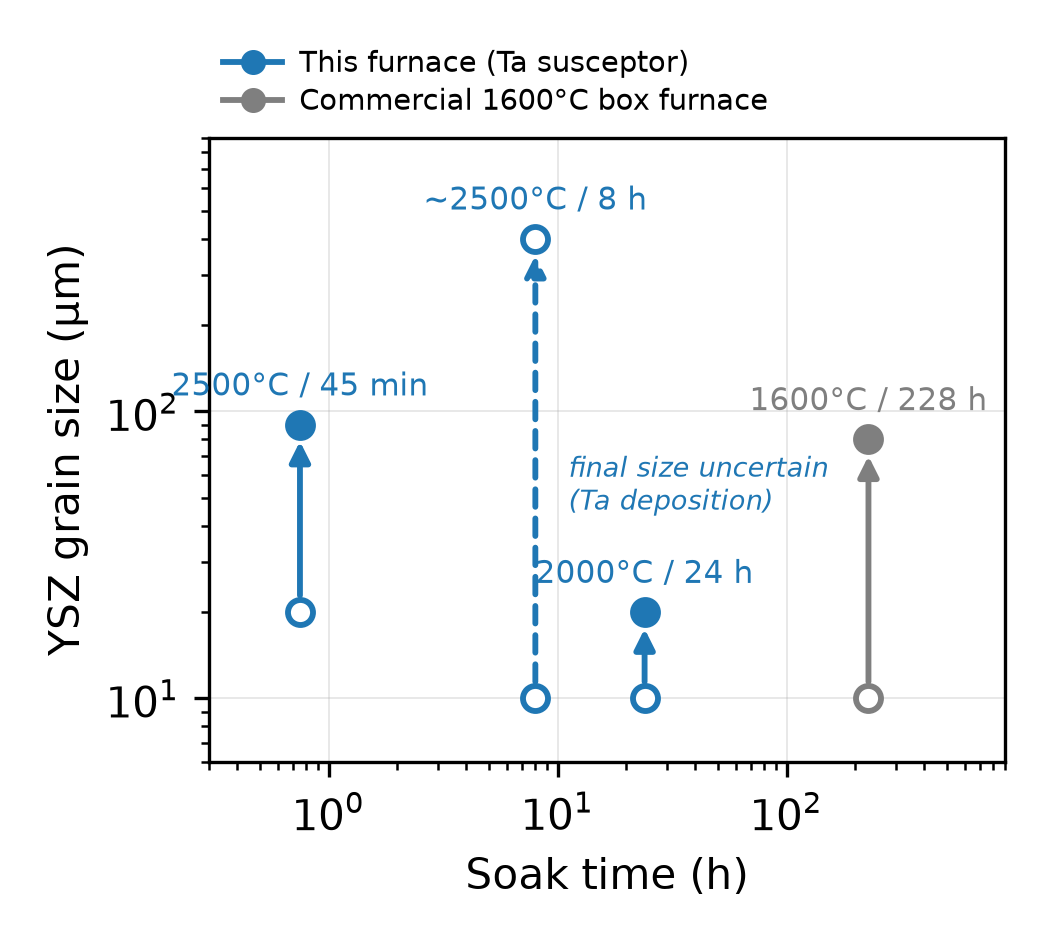
\includegraphics[width=0.66\linewidth]{fig_grain_growth.png}
\caption{As-recorded optical micrograph of the YSZ specimen after the
2500\,\celsius{} / 45\,min tantalum-susceptor anneal, which coarsened the
grains from approximately 20 to 90\,\textmu m. The red multi-grain
measurement traces and the 100\,\textmu m scale bar are part of the original
microscope record.}
\label{fig:graingrowth}
\end{figure}

\begin{figure}[tb]
\centering
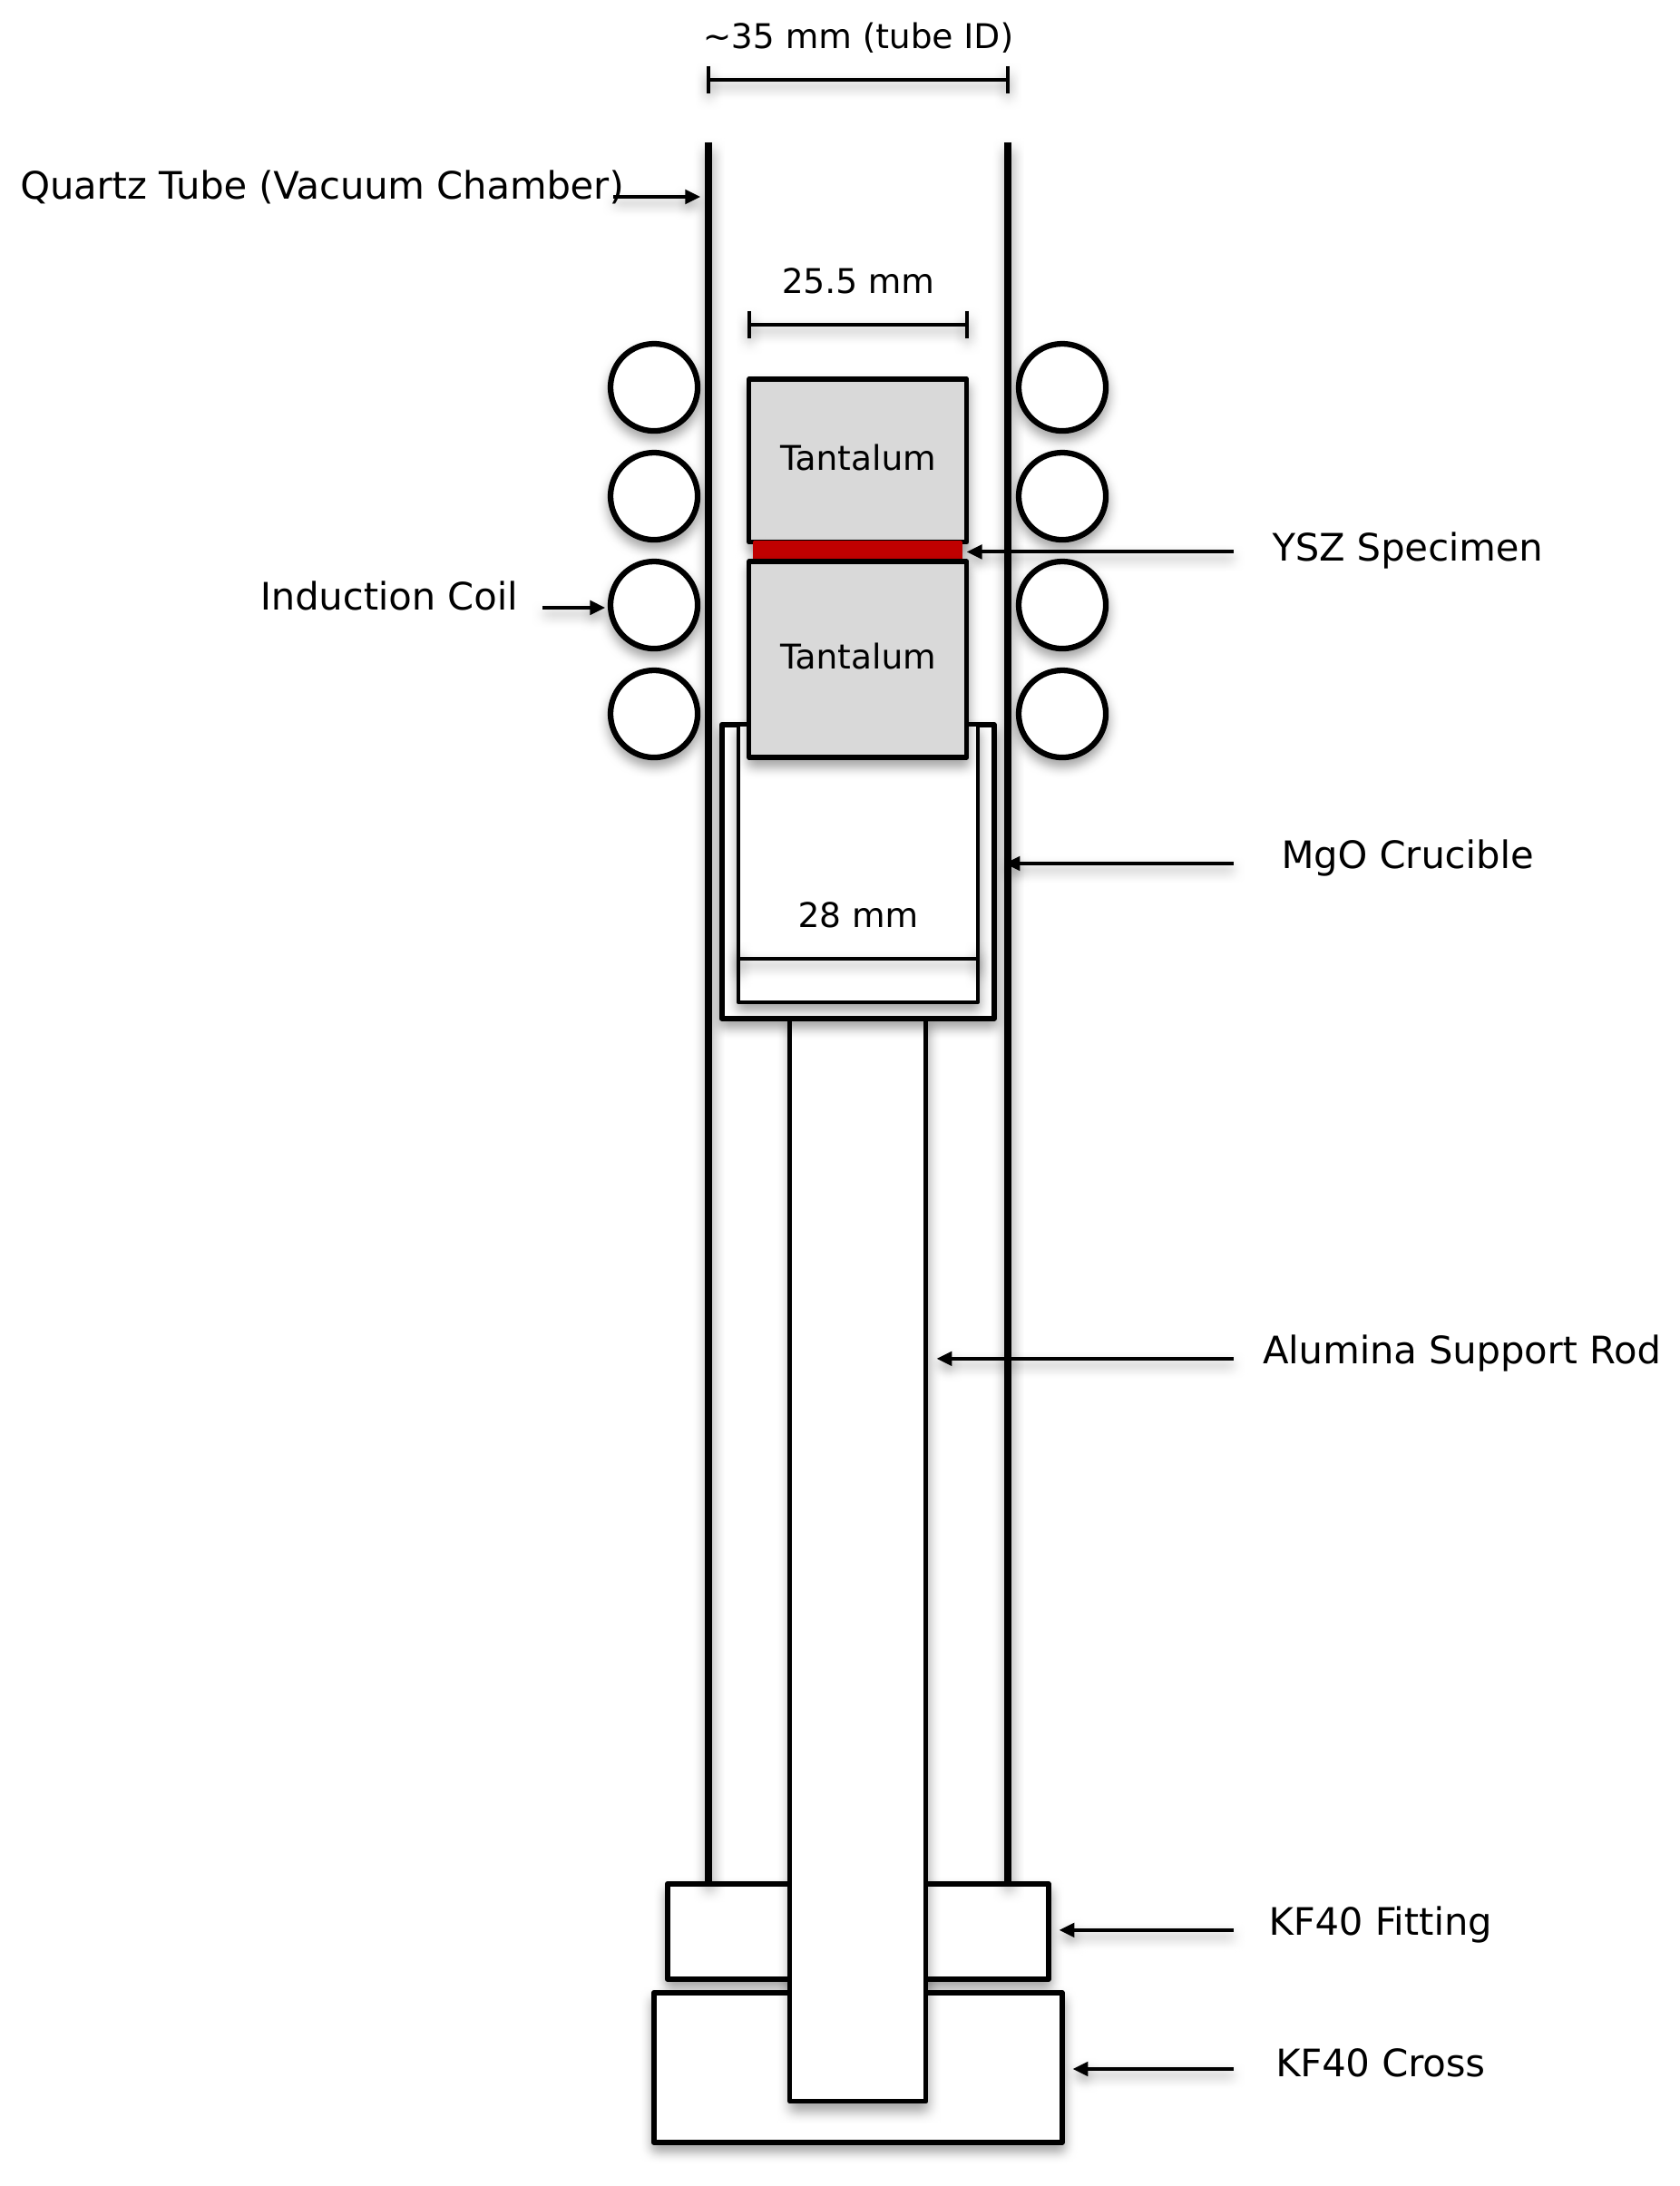
\includegraphics[width=0.46\linewidth]{fig_ysz_stack.png}
\caption{Sample-stack configuration for the high-temperature ceramic
anneals. The YSZ specimen is sandwiched between two 25.5\,mm tantalum
susceptor blocks inside the quartz tube. The blocks rest on a boron nitride
heat-dissipation stub, which sits on the alumina support rod that raises the
sample stack to coil height. The coil, vacuum, pyrometer, and control paths are
unchanged from the metal configuration.}
\label{fig:ysz-stack}
\end{figure}

%==============================================================
\section{Conclusions}
%==============================================================

A bare commercial RF induction generator can be converted into a
computer-controlled, vacuum-integrated, pyrometer-feedback annealing system
with a documented, generator-agnostic modernization stack. On a current
solid-state generator the modernization stack demonstrated a
power--temperature
calibration with $R^2 = 0.991$, high soak repeatability, stable closed-loop
soaks up to 40\,h, and annealed nickel whose surfaces index directly in the
EBSD and show controlled grain growth.

The ceramic extension shows how far the same furnace stretches
without redesign. Exchanging only the materials in contact with the specimen
carries the system from metal anneals in the graphite crucible to ceramic
grain growth at 2500\,\celsius. The trial-and-error survey behind that
result identified chemistry, not
power, as the governing constraint at extreme temperature. Every failure
mode was a contact reaction among the charge, the susceptor, and the
support materials. The interchangeable sample stack lets a user iterate on
those material choices run by run. Because the modernization stack requires
only a
monotonic analog power-control input, the design ports across generators and
is directly reusable at a small fraction of turn-key cost. The
through-thickness boundary grooving points to columnar grain-growth studies
as a natural next application.

%==============================================================
\section*{Supplementary Material}
%==============================================================
% AIP: "Please create a 'Supplementary Material' section in your paper after
% the Conclusions" (template/rsi/aip-author-instructions-2026-07-02.txt).

See the supplementary material for the measured crucible part dimensions,
the work-coil drawing, the power--temperature calibration and the
representative-soak, repeatability, and long-soak traces, the raw
Kikuchi-pattern survey, the tantalum-susceptor heat curves, the YSZ
micrographs, the specimen--thermal-history linkage table with links to
every raw run log, the itemized bill of materials, and the design-file
inventory.

\begin{acknowledgments}
The authors thank Kevin Cole for his supervision and support of the original
retrofit, and acknowledge the BYU Mechanical Engineering Department
and the Johnson group.
\todo{funding sources.}
\end{acknowledgments}

\section*{Author Declarations}

\subsection*{Conflict of Interest}

The authors have no conflicts to disclose. \todo{confirm with all authors.}

\subsection*{Ethics Approval}

This work did not involve human or animal subjects; ethics approval is not
applicable.

\subsection*{Author Contributions}

\todo{confirm CRediT roles} --- provisional: \textbf{Sterling G. Baird:}
Conceptualization, Software, Investigation, Writing -- original draft.
% CRediT mapping of stated contributions: "YSZ grain growth data" ->
% Investigation, Data curation; "procedure" -> Methodology; "photos" ->
% Visualization; "editing" -> Writing - review & editing; O. Johnson (last
% author / PI) -> Supervision, Project administration.
\textbf{Ryan Weber:} Investigation, Methodology, Data curation, Visualization.
\textbf{Christopher Nyborg:} Investigation, Methodology, Data curation,
Visualization.
\textbf{Ronnie Guymon:} Visualization, Writing -- review \& editing.
\textbf{Gage Erickson:} Visualization, Writing -- review \& editing.
\textbf{Oliver Johnson:} Supervision, Project administration.

\section*{Data Availability}

The data that support the findings of this study are openly available in the
development repository
(\url{https://github.com/vertical-cloud-lab/custom-induction-furnace}); an
archival snapshot is deposited at Zenodo,
\href{https://doi.org/10.5281/zenodo.20878017}{https://doi.org/10.5281/zenodo.20878017}.

%==============================================================
% References
%==============================================================
% The bibliography is the validated master reference list compiled from every
% Edison Scientific literature query in this repository (literature-search/),
% de-duplicated and URL/DOI-checked by paper/build_master_bibliography.py.
% REVTeX selects the AIP numeric BibTeX style (aipnum4-2) automatically.
\bibliography{references}

\end{document}
